% ============================================================
% RESULTS SECTION
% ============================================================

\section{Results}\label{sec:results}

We present the evaluation results for all policies across 500 episodes each, focusing on overall performance, SOFA-stratified analysis, and the LEG interpretability comparison that reveals dramatic differences in feature importance patterns across algorithms.

% ============================================================
\subsection{Overall Performance Comparison}\label{sec:results:overall}

Table \ref{tab:overall-performance} and Figure \ref{fig:algorithm-comparison} show results for 8 policies. DDQN-Attention achieves the highest survival at 95.4\%, with all methods in a narrow range from 94.0\% to 95.4\%. Online RL with architectural innovations including DDQN variants and SAC achieves marginally higher rates from 94.2\% to 95.4\% than offline RL methods BC and CQL which range from 94.0\% to 94.2\%. Vanilla DQN at 94.0\% matches offline methods despite online training.

The high baseline survival of approximately 94-95\% across all policies, including the random policy at 95.0\%, reveals that the simulator's outcome model is relatively insensitive to treatment choices. This likely reflects the learned dynamics model's bias toward survival in the underlying MIMIC-III training data, where the majority of patients survived regardless of the specific treatment administered. The random policy's performance matching or exceeding several trained policies does not imply that treatment is irrelevant clinically; rather, it underscores a fundamental limitation of simulator-only evaluation where the outcome model may not capture the true causal effect of treatments on survival. Average returns range from 13.20 to 13.62 with high variance from sparse rewards. Online RL with architectural innovations achieves modest gains of 1.2 to 1.4 percentage points over offline methods yet requires 1M training timesteps, which is infeasible clinically. Offline methods BC and CQL achieve comparable survival of 94.0-94.2\% from pre-collected data only. DQN underperforms on high-severity cases as discussed in Section~\ref{sec:results:sofa}, motivating our focus on interpretability in Section~\ref{sec:results:leg}.

\begin{table}[htbp]
\centering
\caption{Overall performance across 500 evaluation episodes. Bold values indicate the highest performance in each column.}
\label{tab:overall-performance}
\begin{tabular}{lcccc}
\toprule
\textbf{Model} & \textbf{Survival (\%)} & \textbf{Avg Return} & \textbf{Avg Length} & \textbf{Training} \\
\midrule
\multicolumn{5}{l}{\textit{Baselines}} \\
Random          & 95.0               & 13.50 $\pm$ 6.54    & 9.3 $\pm$ 1.1       & -- \\
Heuristic       & 94.6               & 13.38 $\pm$ 6.78    & 9.5 $\pm$ 1.2       & -- \\
\midrule
\multicolumn{5}{l}{\textit{Offline RL (trained on 2,105 episodes, approximately 20K transitions)}} \\
BC              & 94.2               & 13.26 $\pm$ 7.01    & 9.5 $\pm$ 0.6       & Offline \\
CQL             & 94.0               & 13.20 $\pm$ 7.12    & 9.5 $\pm$ 0.5       & Offline \\
\midrule
\multicolumn{5}{l}{\textit{Hybrid Baseline (vanilla Q-learning, online trained)}} \\
DQN             & 94.0               & 13.20 $\pm$ 7.12    & 7.8 $\pm$ 1.2       & Online$^\dagger$ \\
\midrule
\multicolumn{5}{l}{\textit{Online RL (trained via 1M timesteps of simulator interaction)}} \\
DDQN-Attention  & \textbf{95.4}      & 13.62 $\pm$ 6.28    & 7.9 $\pm$ 1.0       & Online \\
DDQN-Residual   & 94.2               & 13.26 $\pm$ 7.01    & 9.0 $\pm$ 0.8       & Online \\
SAC             & 94.8               & 13.44 $\pm$ 6.66    & 7.7 $\pm$ 1.2       & Online \\
\bottomrule
\end{tabular}
\begin{flushleft}
\scriptsize
Note: BC and CQL are trained offline on 2,105 episodes (approximately 20K transitions). Online methods (DDQN variants and SAC) train via 1M timesteps of simulator interaction. \\
$^\dagger$DQN: foundational online Q-learning baseline lacking offline constraints from CQL or architectural innovations from DDQN-Attention/Residual and SAC. \\
Avg = Average.
\end{flushleft}
\end{table}

\begin{figure}[htbp]
\centering

\includegraphics[width=\textwidth]{../results/figures/algorithm_comparison.png}
\caption{Performance comparison across all algorithms. Top left: survival rates; top right: average returns; bottom left: SOFA-stratified survival; bottom right: episode lengths.}
\label{fig:algorithm-comparison}
\end{figure}


% ============================================================
\subsection{SOFA-Stratified Analysis}\label{sec:results:sofa}

We stratified episodes by SOFA score into low ($\leq$5), medium (6-10), and high ($\geq$11) categories. All methods exceed 97\% on low and medium severity cases, reflecting a ceiling effect. Table \ref{tab:sofa-stratified} shows high-SOFA results. DDQN-Attention achieves the highest survival at 90.5\%, with a 1.9 percentage point advantage over BC and CQL at 88.6\% and 88.5\% respectively. Offline methods BC and CQL match SAC at 88.7\% but substantially outperform DQN at 84.3\%. CQL combines competitive high-SOFA performance with superior interpretability as shown in Section~\ref{sec:results:leg}.

\begin{table}[htbp]
\centering
\caption{Performance on high-severity patients (SOFA $\geq$ 11). Bold values indicate the highest survival rate.}
\label{tab:sofa-stratified}
\begin{tabular}{lcccc}
\toprule
\multicolumn{5}{c}{\textbf{High SOFA ($\geq$ 11) - Most Severe Patients}} \\
\midrule
\textbf{Model} & \textbf{$n$} & \textbf{Survival (\%)} & \textbf{Avg Return} & \textbf{Avg Length} \\
\midrule
\multicolumn{5}{l}{\textit{Offline RL}} \\
BC              & 211 & 88.6 & 11.63 $\pm$ 9.82  & 8.3 $\pm$ 1.1 \\
CQL             & 191 & 88.5 & 11.55 $\pm$ 9.95  & 8.3 $\pm$ 1.1 \\
\midrule
\multicolumn{5}{l}{\textit{Hybrid Baseline}} \\
DQN             & 185 & 84.3 & 10.29 $\pm$ 11.46 & 8.5 $\pm$ 1.2 \\
\midrule
\multicolumn{5}{l}{\textit{Online RL}} \\
DDQN-Attention  & 190 & \textbf{90.5} & 12.16 $\pm$ 8.79  & 8.0 $\pm$ 1.1 \\
DDQN-Residual   & 200 & 87.0 & 11.10 $\pm$ 10.09 & 8.3 $\pm$ 1.2 \\
SAC             & 195 & 88.7 & 11.62 $\pm$ 9.49  & 8.1 $\pm$ 1.1 \\
\bottomrule
\end{tabular}
\begin{flushleft}
\scriptsize
Note: $n$ = sample size for each algorithm in the high-SOFA stratum. Avg = Average.
\end{flushleft}
\end{table}


% ============================================================
\subsection{LEG Interpretability Analysis}\label{sec:results:leg}

We now present the core contribution of this work: a systematic comparison of interpretability across all 6 algorithms, comprising 3 offline methods including BC, CQL, and DQN, and 3 online methods including DDQN-Attention, DDQN-Residual, and SAC, using Linearly Estimated Gradients analysis. We analyzed 10 representative states per algorithm using identical parameters with 1,000 perturbation samples and $\sigma=0.1$, sampled uniformly across SOFA severity levels, and computed feature importance scores for the action selected by each policy. The results reveal dramatic differences in interpretability magnitude spanning 3 orders of magnitude, with profound implications for the offline-vs-online trade-off and clinical deployment.

\subsubsection{Feature Importance Magnitude Comparison}

Table \ref{tab:interpretability-metrics} and Figure \ref{fig:leg-6model} summarize the LEG interpretability metrics for all 6 algorithms. The most striking finding is the maximum saliency magnitude, which quantifies the strength of the strongest feature importance signal. CQL achieves the highest saliency with a maximum of 40.06 for systolic blood pressure, suggesting strong dependence on a clinically relevant hemodynamic marker. The 3 online RL methods exhibit intermediate saliency, with DDQN-Attention achieving 3.57 for qSOFA, DDQN-Residual achieving 2.93 for INR, and SAC achieving 1.17 for INR. The remaining offline methods show weaker signals. BC achieves 0.78, and DQN exhibits the weakest signal at 0.069, representing an approximately 580-fold difference compared to CQL (40.06 / 0.069 = 581). While we lack validated benchmarks to define absolute interpretability thresholds, this 3-order-of-magnitude range demonstrates substantial algorithmic variation in feature importance strength.

This 3-order-of-magnitude range reveals a clear interpretability hierarchy. Conservative offline RL as represented by CQL ranks highest, followed by online RL with architectural innovations such as DDQN-Attention and DDQN-Residual, then online RL without structure as represented by SAC, then imitation learning as represented by BC, and finally online-trained DQN at the bottom. Online methods achieve 11-fold weaker interpretability than CQL at 40.06 vs. 3.57 despite marginally higher survival rates of 95.4\% vs. 94.0\%, demonstrating a measurable performance-interpretability trade-off. However, online methods remain 50-fold more interpretable than vanilla DQN at 3.57 vs. 0.069, suggesting that architectural choices such as attention mechanisms and residual connections can partially mitigate the interpretability loss from online training.

The interpretability patterns reflect algorithmic differences in representation learning. CQL's conservatism biases the Q-function toward simple, threshold-based structures aligned with the heuristic behavioral policy, yielding strong gradients on clinically relevant features such as blood pressure and lactate. Online methods with attention and residual architectures preserve moderate interpretability by learning structured feature weighting, with DDQN-Attention's top feature being qSOFA which aligns with clinical severity scoring. In contrast, DQN's unconstrained deep network learns highly non-linear representations where no single feature dominates, producing uniformly weak saliency scores unsuitable for clinical validation.

\begin{figure}[htbp]
\centering
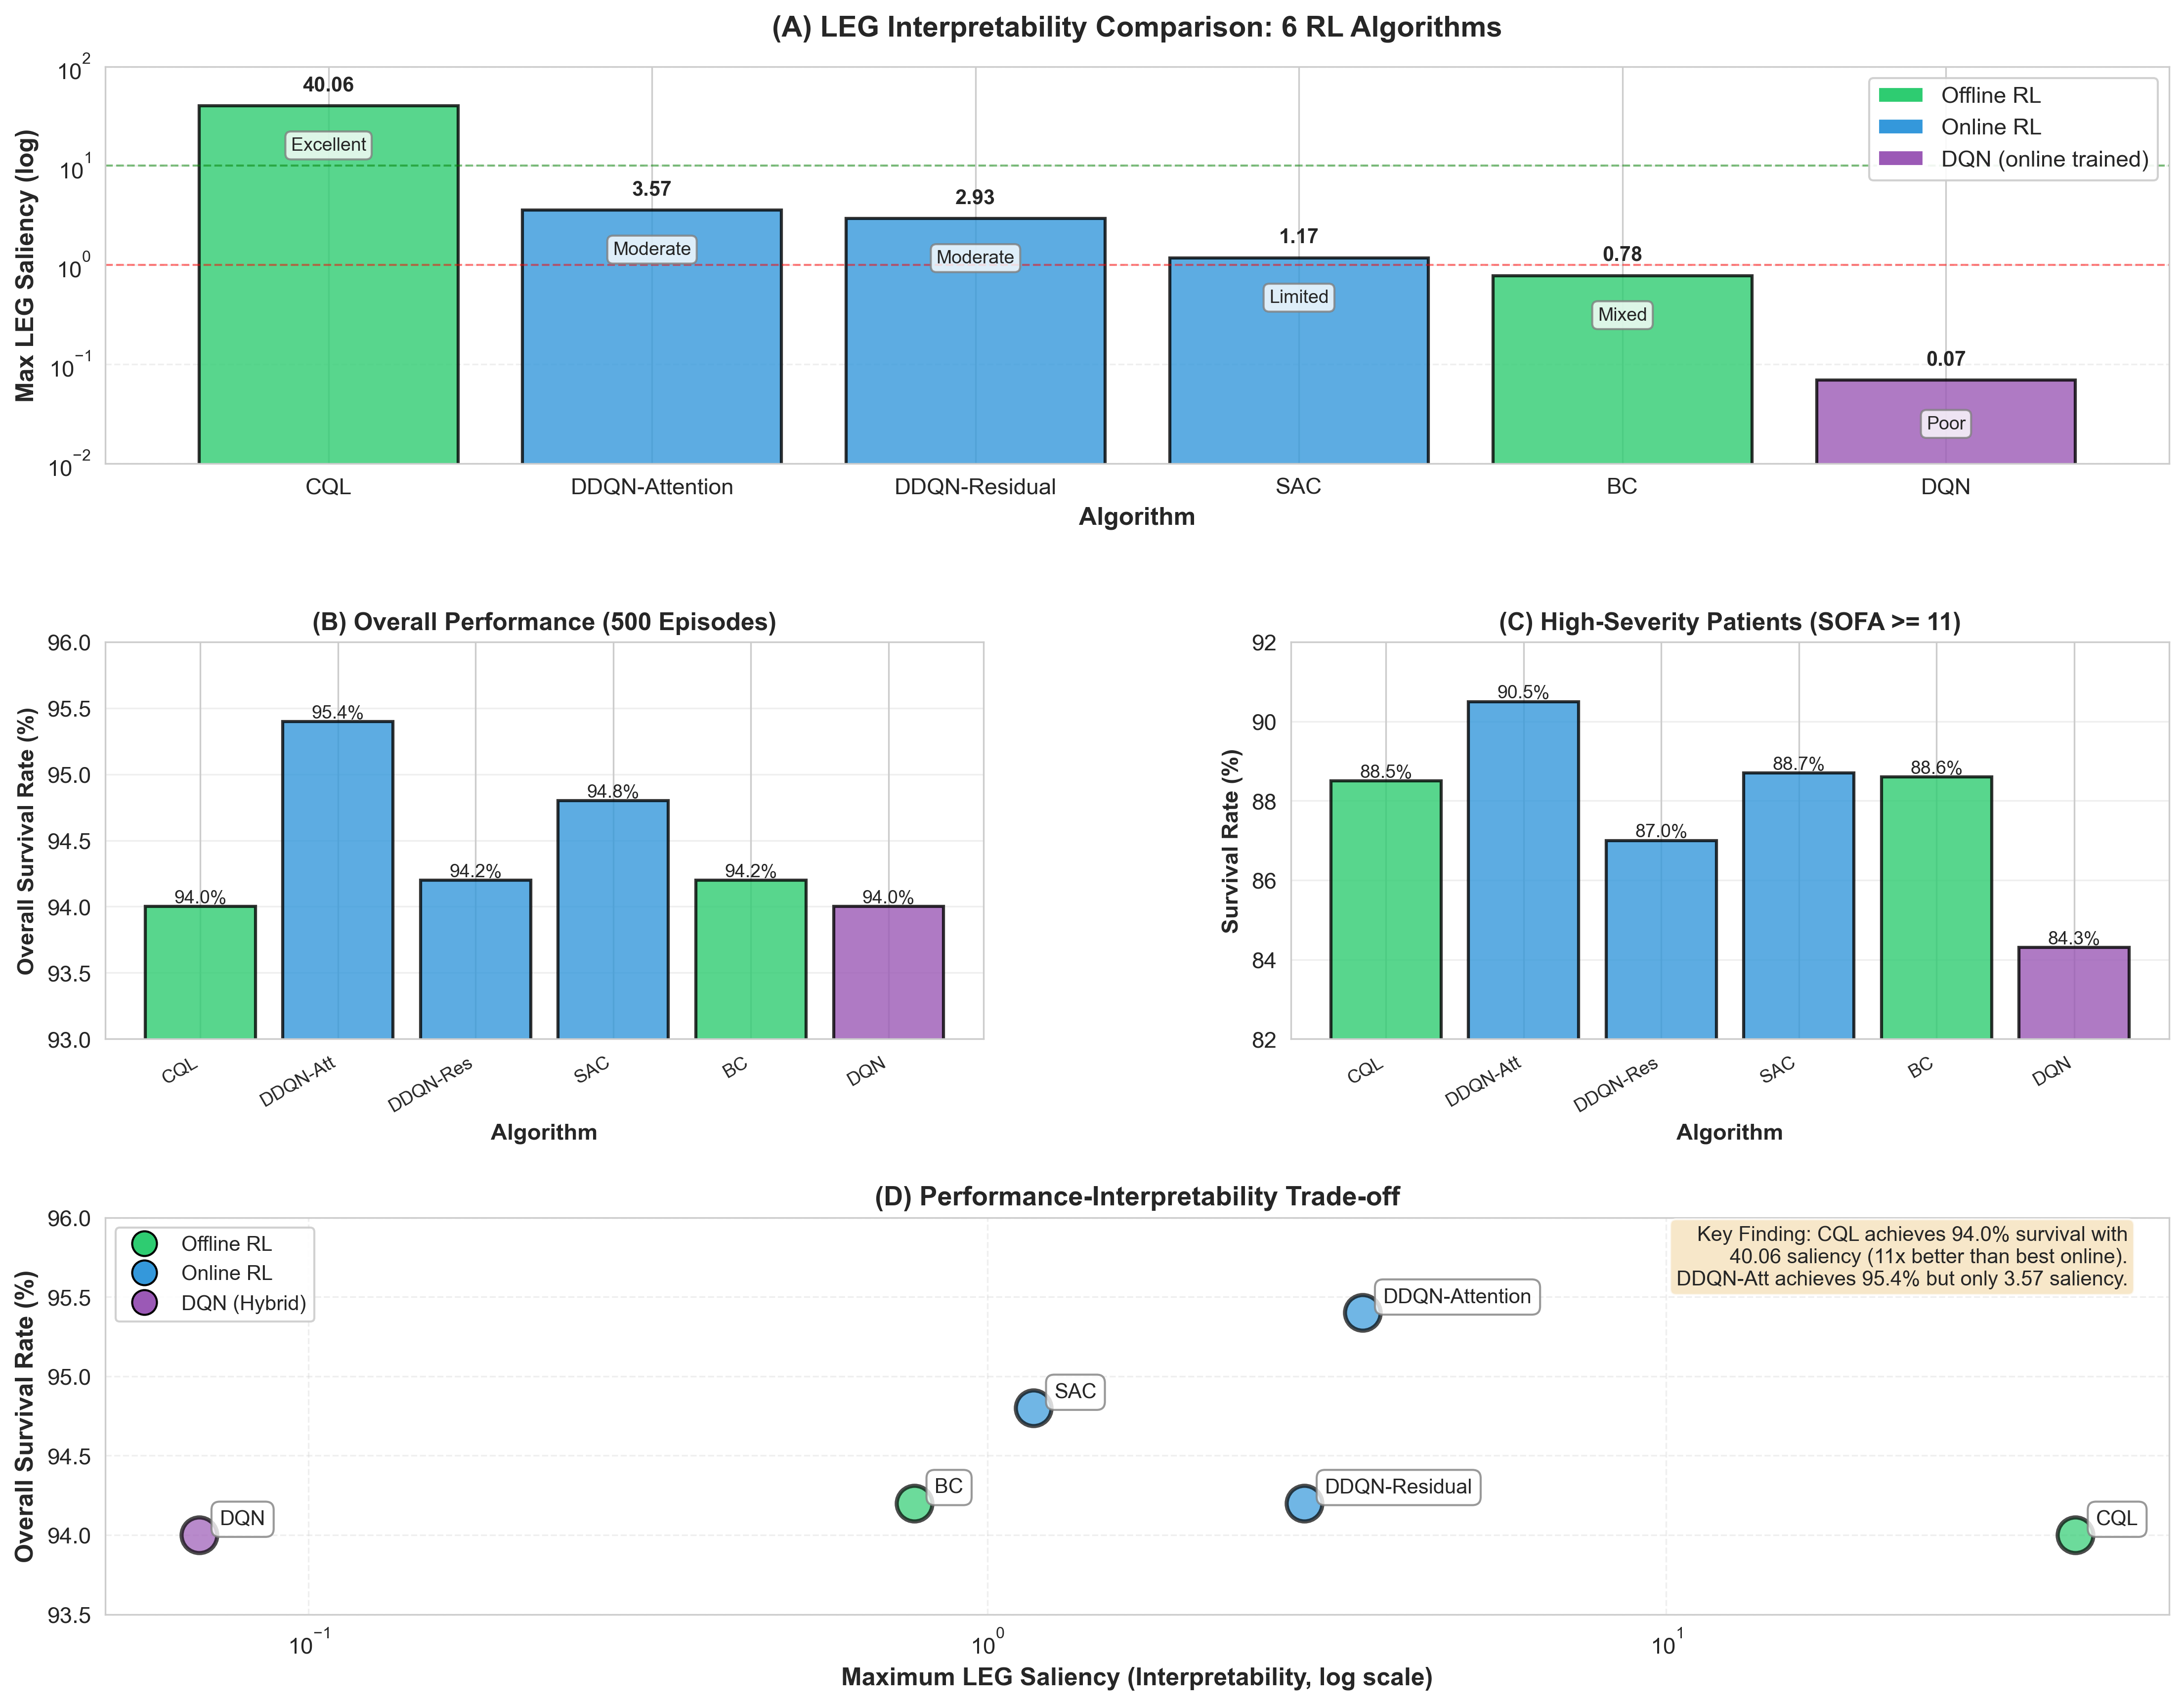
\includegraphics[width=\textwidth]{../results/figures/leg_6model_comparison.png}
\caption{Comprehensive 6-model LEG interpretability analysis. Top: maximum saliency scores on logarithmic scale showing 3 orders of magnitude variation from CQL at 40.06 to DQN at 0.069. Middle: performance comparison of survival rates. Bottom: performance-saliency trade-off scatter plot.}
\label{fig:leg-6model}
\end{figure}

\begin{table}[htbp]
\centering
\caption{LEG interpretability metrics for all 6 algorithms with 10 representative states each using identical parameters of $n=1000$ and $\sigma=0.1$. CQL achieves 11-fold stronger saliency than the best online method DDQN-Attention and approximately 580-fold stronger than vanilla DQN. Saliency magnitude is a proxy for feature-driven decision-making but does not guarantee clinical trust without prospective validation. Training paradigm labels are Offline for fixed dataset, Hybrid for online-trained vanilla Q-learning baseline, and Online for simulator interaction with architectural innovations.}
\label{tab:interpretability-metrics}
\begin{tabular}{lcccc}
\toprule
\textbf{Algorithm} & \textbf{Training} & \textbf{Max Saliency} & \textbf{Top Feature} & \textbf{Clinical Coherence$^\ddagger$} \\
\midrule
CQL                & Offline  & 40.06  & SysBP    & High (hemodynamic) \\
DDQN-Attention     & Online   & 3.57   & qSOFA    & High (severity score) \\
DDQN-Residual      & Online   & 2.93   & INR      & Mixed (coagulation) \\
SAC                & Online   & 1.17   & INR      & Mixed (coagulation) \\
BC                 & Offline  & 0.78   & qSOFA    & High (severity score) \\
DQN                & Hybrid$^\dagger$  & 0.069  & INR      & Weak (low signal) \\
\bottomrule
\multicolumn{5}{l}{\scriptsize $^\dagger$DQN: vanilla online-trained Q-learning baseline; see Section~\ref{sec:discussion:limitations}} \\
\multicolumn{5}{l}{\scriptsize $^\ddagger$Clinical coherence: qualitative assessment of alignment with medical guidelines} \\
\end{tabular}
\end{table}


\subsubsection{Clinical Implications and Algorithm Selection}

The 6-model LEG comparison reveals that interpretability is not uniformly sacrificed for performance. CQL's conservative value estimation biases the Q-function toward threshold-based logic mirroring the heuristic behavioral policy, yielding strong gradients on clinically relevant features such as SysBP, lactate, and MeanBP aligned with Surviving Sepsis Campaign guidelines \citep{rhodes2017ssc}. Online methods with architectural innovations including DDQN-Attention's multi-head attention and DDQN-Residual's skip connections preserve moderate interpretability by learning structured feature weighting, with top features qSOFA and INR aligning with clinical severity markers. In contrast, vanilla DQN's unconstrained deep network learns distributed representations with uniformly weak, clinically incoherent saliency patterns.

For clinical deployment, this hierarchy suggests several recommendations. Conservative offline RL as implemented in CQL offers the optimal balance with competitive survival of 94.0\% overall and 88.5\% high-SOFA, exceptional interpretability with 40.06 saliency, and no patient risk during training. Online RL with attention as implemented in DDQN-Attention achieves marginally better survival at 95.4\% overall and 90.5\% high-SOFA but requires 11-fold interpretability sacrifice and environment interaction infeasible in clinical settings. Behavior cloning and vanilla DQN exhibit poor or inconsistent interpretability unsuitable for regulatory approval. The finding that CQL achieves both strong performance and exceptional interpretability demonstrates that the performance-interpretability trade-off is not inevitable. Conservatism in the learning objective enables simultaneously effective and explainable policies.

% End of Results section
